\documentclass[12pt]{beamer}
\author{}
\title{Paper Reading Seminar}
\subtitle{}
\usetheme{Malmoe}
\setbeamertemplate{navigation symbols}{}
\newcommand*\oldmacro{}%
\let\oldmacro\insertshorttitle%
\renewcommand*\insertshorttitle{%
\oldmacro\hfill%
\insertframenumber\,/\,\inserttotalframenumber}

\usefonttheme{professionalfonts}

\begin{document}

\begin{frame}[plain]
	\titlepage
\end{frame}

\begin{frame}{Overview of the paper review}
	\begin{itemize}
		\item We only care about
		\begin{itemize}
			\item (Are there already standard approaches?)
			\item How do they define the problem and the objective?
			\item Why is this problem challenging?
			\item How do the other researchers solve them?
		\end{itemize}
		\item $\Rightarrow$ We don't review the experiment sections here
	\end{itemize}
\end{frame}

\begin{frame}{Paper 1}
	\begin{itemize}
		\item Fernando de la Torre et. al. Temporal Segmentation of Facial Behavior, ICCV 2007 
	\end{itemize}
\end{frame}

\begin{frame}{Problem definition}
	\begin{itemize}
		\item Temporal segmentation of facial behavior
		\item The authors don't give a specific definition. And my understanding is
		\begin{itemize}
			\item The result segments are expected to be similar within themselves, but different between each other
			\item Elements in each segment should be continuous in time
			\item There may also be classification involved considering this paper is also about facial expressions
		\end{itemize}
	\end{itemize}
\end{frame}

\begin{frame}{Challenges}
	\begin{itemize}
		\item Mainly the unreliability of face tracking
		\begin{itemize}
			\item Non-frontal pose
			\item Moderate out-of-plane head motion
			\item Subtle facial actions
		\end{itemize}
		\item Also some challengings in the algorithm aspect
		\begin{itemize}
			\item Large variability in the temporal scale
		\end{itemize}
	\end{itemize}
\end{frame}

\begin{frame}{Approach}
	\begin{itemize}
		\item Goal
		\begin{itemize}
			\item Robust to 2D affine transforms
			\item (Background introduction: geometric transforms and RANSAC)
		\end{itemize}
	\end{itemize}
\end{frame}

\begin{frame}{Approach}
	\begin{itemize}
		\item Framework: feature clustering + temporal clustering (process individually)
		\item Feature clustering
		\begin{itemize}
			\item Feed pairwise similarity to \emph{spectral clustering}
			\item (Background introduction: graph-cut and normalized-cut)
			\item Distance computation: consider 2D transforms
			\begin{itemize}
				\item Point coordinates $S_1, S_2 \Rightarrow H$
				\item Dist $= \mathcal{N}(s_i - Hs_j) \mathcal{N}(h_i - h_j)$
			\end{itemize}
		\end{itemize}
	\end{itemize}
\end{frame}

\begin{frame}{Approach}
	\begin{itemize}
		\item Temporal clustering
		\begin{itemize}
			\item Biased (natural) pose detection and elimination
			\begin{itemize}
				\item Facial temporal clustering is special because it has a biased/natural pose
				\item Frames =HMM=$>$ ``static'' poses =Spectral Clustering=$>$ natural poses
			\end{itemize}
		\end{itemize}
	\end{itemize}
\end{frame}

\begin{frame}{Approach}
	\begin{itemize}
		\item Details about HMM
		\\ \medskip { 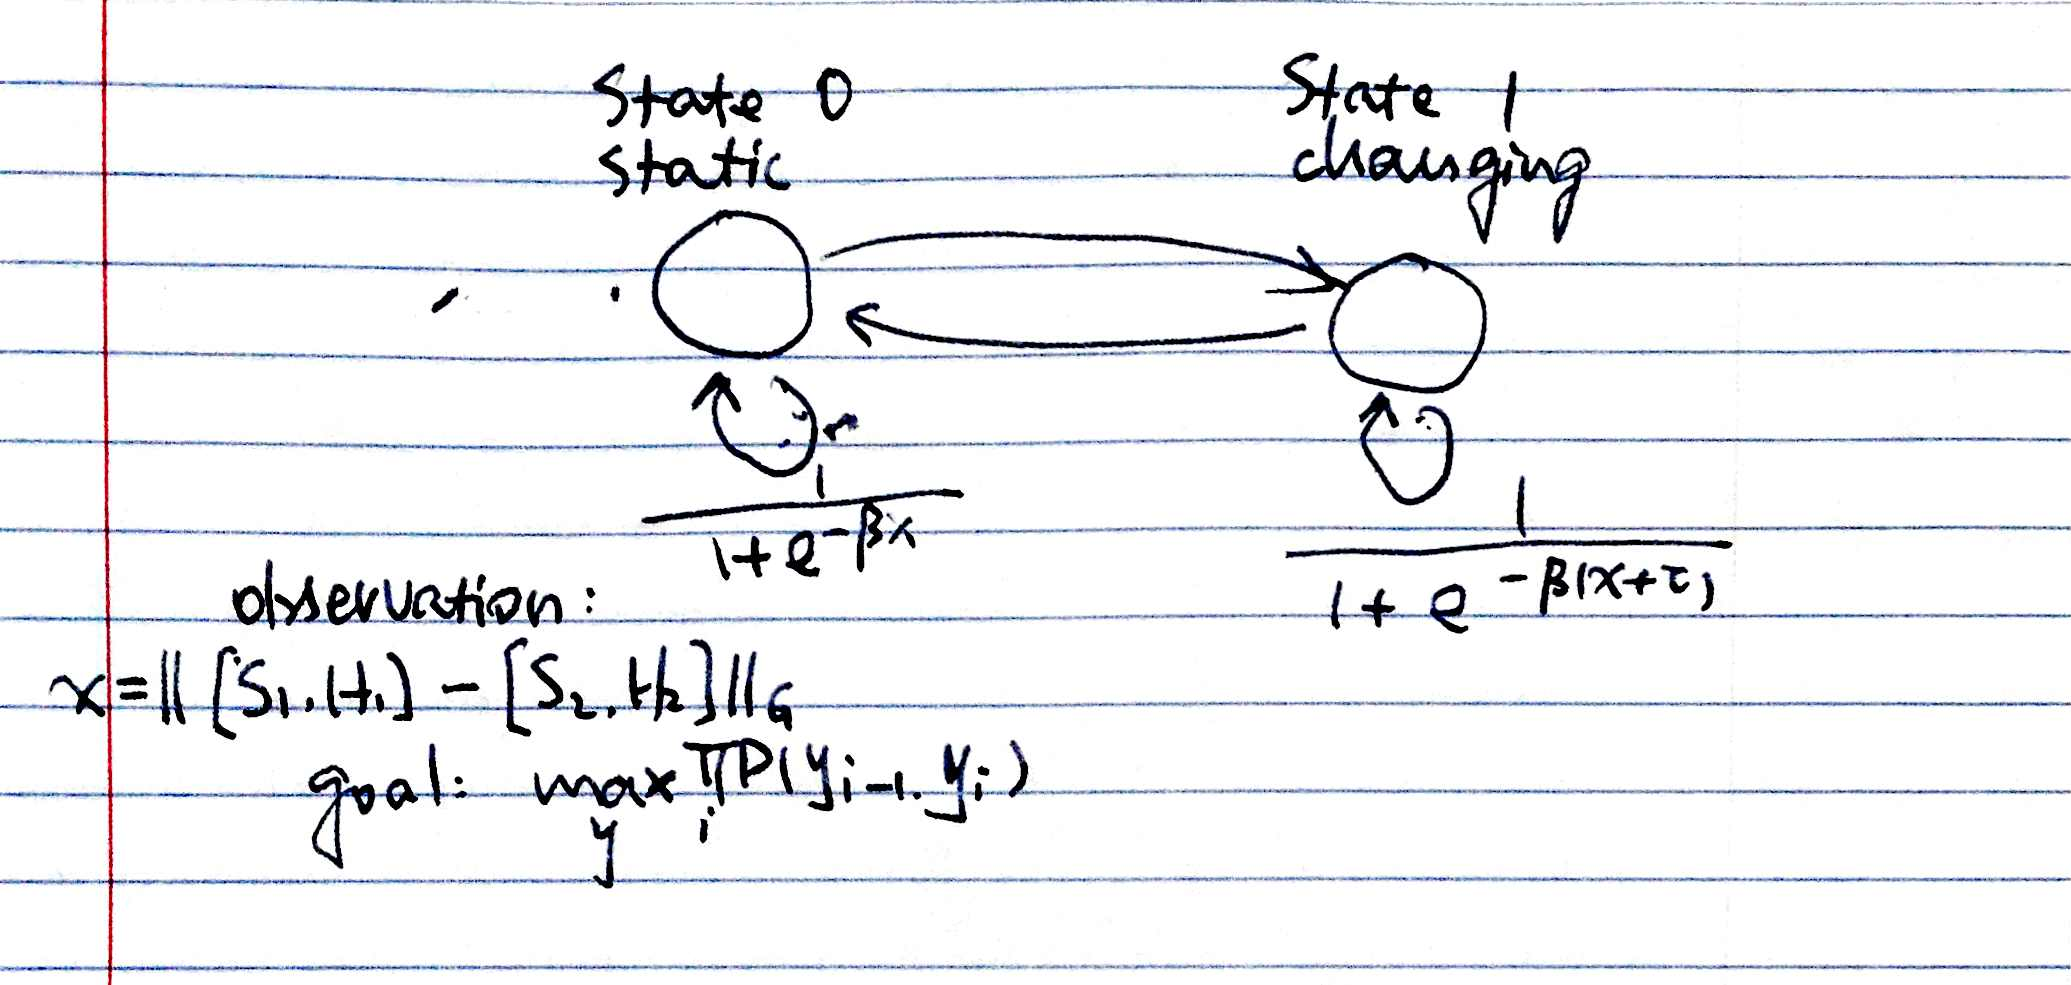
\includegraphics[width=0.9\textwidth]{hmm.jpg} \\ } 
	\end{itemize}
\end{frame}

\begin{frame}{Approach}
	\begin{itemize}
		\item Details about HMM
		\\ \medskip { 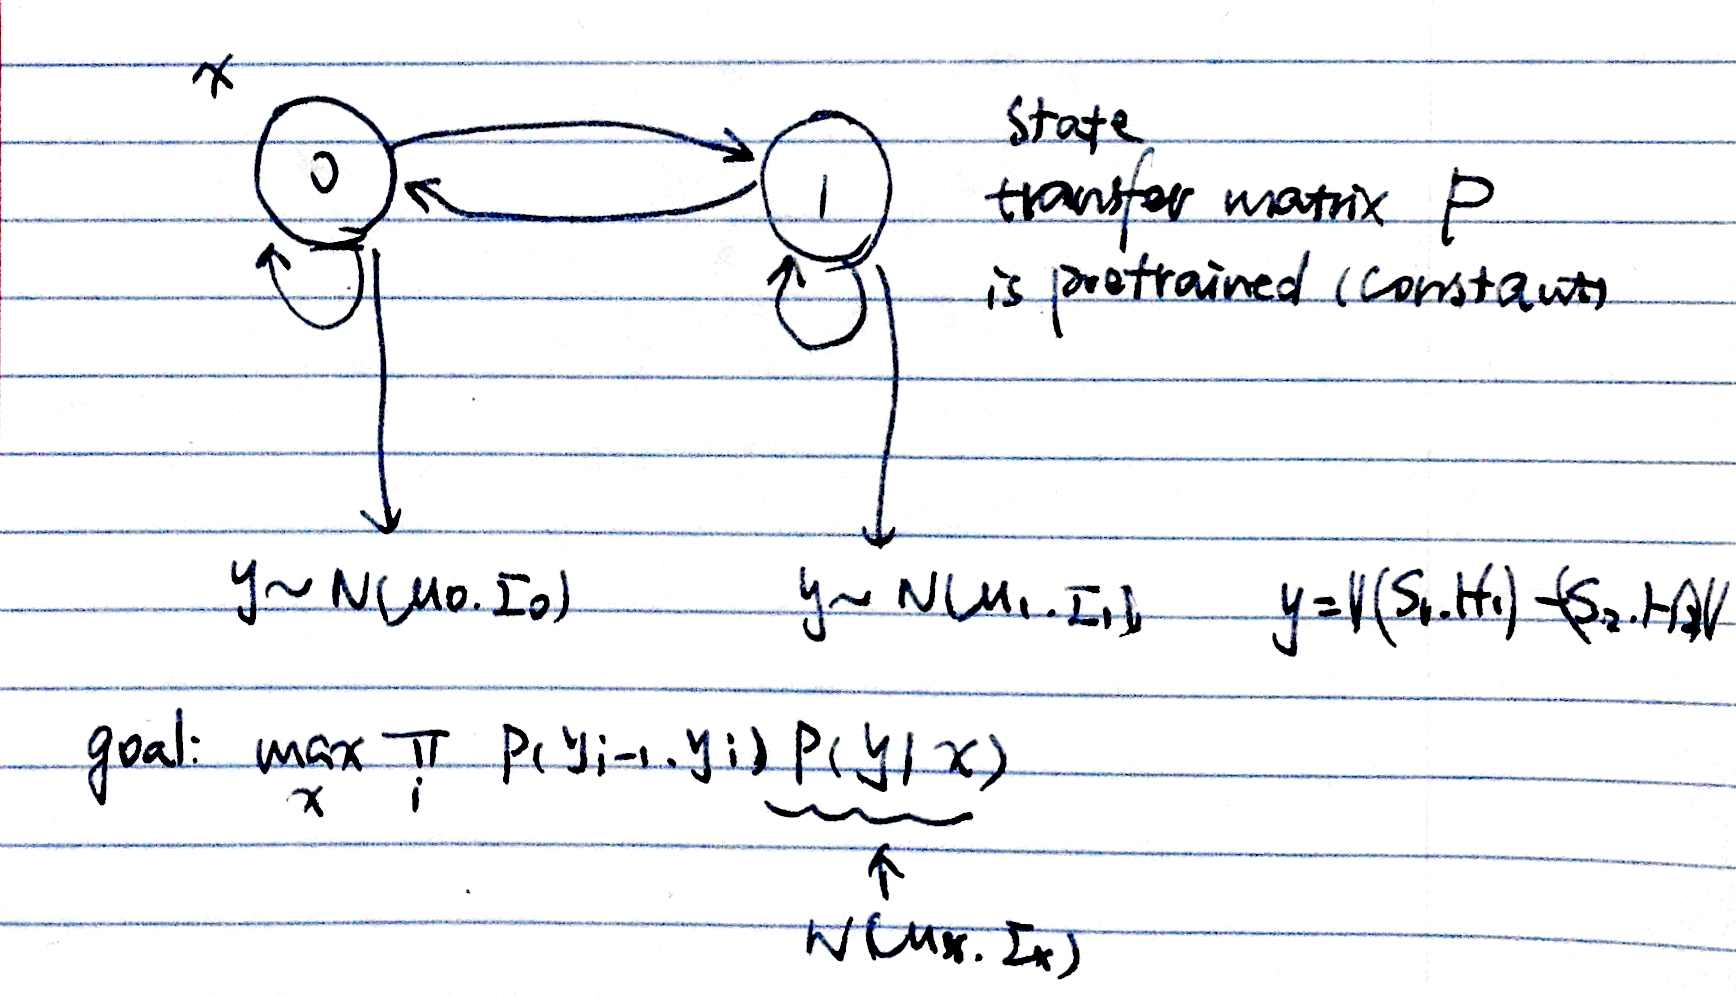
\includegraphics[width=0.9\textwidth]{hmm_correct.jpg} \\ } 
	\end{itemize}
\end{frame}

\begin{frame}{Approach}
	\begin{itemize}
		\item Clustering of other poses
		\begin{itemize}
			\item Temporal greedy scanning
			\\ \medskip { 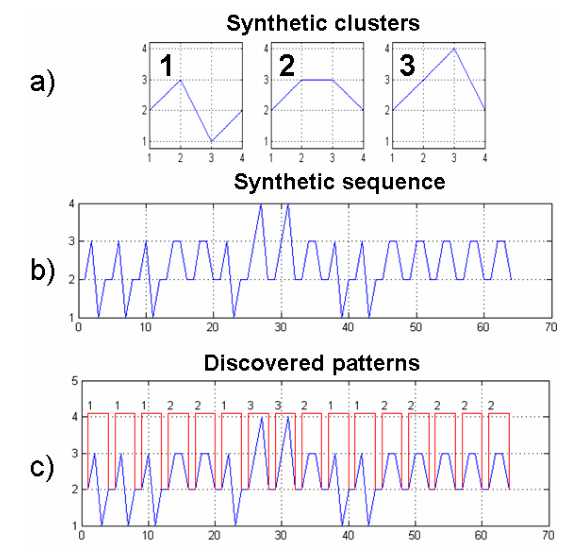
\includegraphics[width=0.55\textwidth]{scanning.png} \\ } 
		\end{itemize}
	\end{itemize}
\end{frame}

\begin{frame}{Some thoughts}
	\begin{itemize}
		\item HMM looks a slightly better version of feature difference thresholding
		\item The overall framework is just greedy matching, while largest cluster gets double-confirmed by HMM
        \begin{itemize}
        	\item Our first baseline?
        \end{itemize}
		\item Feature clustering may act as an intermediate representation
		\begin{itemize}
			\item May be sensitive. Let's first test whether it has real-world meanings...
		\end{itemize}
		\item Greedy scanning may act as our first baseline?
		\begin{itemize}
			\item Can track papers citing this paper to for other baselines
		\end{itemize}
        \item HMM may be an interesting direction to pursue? (with efficient max-margin inference?)
	\end{itemize}
\end{frame}

\begin{frame}{Paper 2}
	\begin{itemize}
		\item Minh Hoai, Fernando de la Torre, Maximum Margin Temporal Clustering, AISTATS 2012
	\end{itemize}
\end{frame}

\begin{frame}{Problem definition}
	\begin{itemize}
		\item Factorization of multiple time series into a set of non-overlapping segments that belongs to $k$ temporal clusters
		\item Previous work
		\begin{itemize}
			\item Hidden Morkov Model
			\item Dynamic Bayesian Network
			\item Support Vector Machine
		\end{itemize}
		\item The related work section is very useful
	\end{itemize}
\end{frame}

\begin{frame}{Multi-class Max Margin Clustering}
	\begin{itemize}
		\item Background introduction: SVM)
		\[ \begin{aligned}[rl] \min & \frac{1}{2m} \sum_j \lVert w_j \rVert^2 + C\sum_i \xi_i \\ \text{s.t. } & \forall i: w_{y'}^Tx_i - w_y^Tx_i \geq 1 - \xi_i, \forall y \neq y' \\ & \forall j, j': -\lambda \leq (w_j - w_{j'})^T\sum_i x_i \leq \lambda \end{aligned} \]
		\item Cluster balance?
	\end{itemize}
\end{frame}

\begin{frame}{Membership requirement MMC}
	\begin{itemize}
		\item Formulation
        \[ \begin{aligned}[rl] \min & \frac{1}{2m} \sum_j \lVert w_j \rVert^2 + C\sum_i \xi_i + C_2\sum_j \beta_j \\ \text{s.t. } & \forall i: w_{y'}^Tx_i - w_y^Tx_i \geq 1 - \xi_i, \forall y \neq y' \\ & \forall j: \exists l \text{ different indexers }i\text{s}: \\ & w_j^Tx_i-w_{j'}^Tx_i\geq1-\beta_j, \forall j' \neq j \end{aligned} \]
		\item Soft constraint requiring each cluster to have at least $l$ members
		\item Optimize with coordinate descent
	\end{itemize}
\end{frame}

\begin{frame}{Joint segmentation and clustering}
	\begin{itemize}
		\item Adding changing points $\{s_i\}$ (heuristic)
		\\ \medskip { 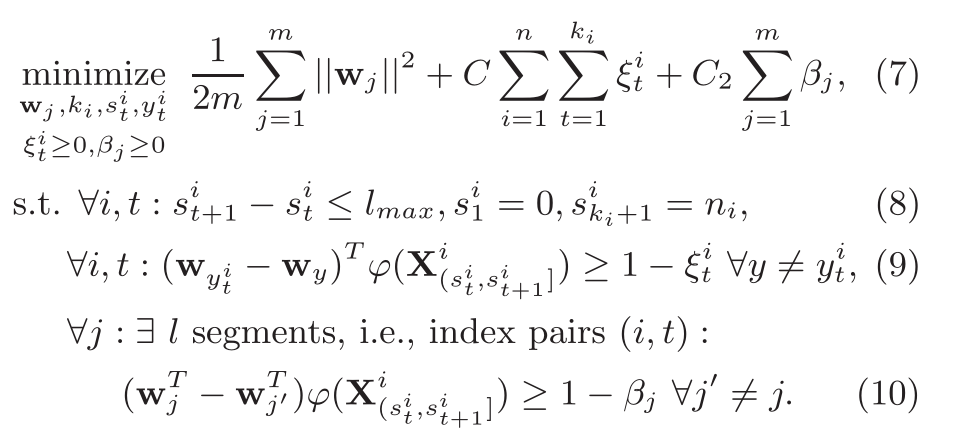
\includegraphics[width=0.9\textwidth]{mmtc.png} \\ } 
		\item Optimize with block coordinate descent and alternating optimization
	\end{itemize}
\end{frame}

\begin{frame}{Some thoughts}
	\begin{itemize}
		\item Large-margin approaches is appealing in that it also selects the important features (especially with $l_1$ norms)
		\item The training process may be troublesome, requiring upper bound approximation and cutting-plane optimization. But may also bring more technical contributions
	\end{itemize}
\end{frame}

\end{document}